\section{Métodos no supervisados}
\begin{frame}{Métodos no supervisados}
\begin{columns}
\begin{column}{0.9\textwidth}
Los métodos no supervisados son aquellos que buscan analizar la estructura subyacente de los datos. De esta manera no hay una diferenciación de variables, sino que se analizan las relaciones entre las variables. 
\end{column}
\end{columns}
\end{frame}


\subsection{Análisis de componentes principales}
\begin{frame}{Métodos no supervisados}
\begin{columns}
\begin{column}{0.9\textwidth}
Dado un vector aleatorio $\mathbf{x}$ de longitud $p$. Sea $r=rg(\mathbf{X})$. Entonces se definen las componentes principales:
\begin{defi}
Se definen las componentes principales 
\begin{equation}
Z_j=v_{1j}X_1+\ldots v_{pj}X_p=\mathbf{v}_j^T\mathbf{x}^T \quad j=1\ldots r
\end{equation}

\noindent Donde $\textbf{v}_j$ es un vector columna con $p$ escalares y la nueva variable aleatoria $Z_j$ cumple lo siguiente:
\begin{itemize}
\item Si $j=1$ $Var(Z_1)$ es máxima restringido a $\mathbf{v}_1^T \mathbf{v}_1=1$
\item Si $j>1$ debe cumplir:
\begin{itemize}
\item $Cov(Z_j,Z_i)=0\quad \forall i\neq j $
\item $\textbf{v}_j^T \textbf{v}_j=1$
\item $Var(Z_j)$ es máxima. 
\end{itemize}
\end{itemize}
\end{defi}
\end{column}
\end{columns}
\end{frame}


\begin{frame}{Métodos no supervisados}
\begin{columns}
\begin{column}{0.9\textwidth}
\begin{defi}
Dada una matriz $\textbf{X}\in  \mathbb{M}_{N\times p}(\mathbb{R})$ existe la descomposición en valores singulares :
\begin{equation}
\textbf{X}=\textbf{U}\mathbf{D}\textbf{V}^T
\end{equation}
Donde: 
\begin{itemize}
\item \textbf{U} matriz ortogonal y de tamaño $N \times r$
\item $\mathbf{D}$ matriz de tamaño $r \times r$ diagonal, cuyos elementos no nulos son los valores singulares $\sigma_1\geq\ldots\geq \sigma_r\geq 0$, es decir
\begin{equation}
\mathbf{D}=\begin{pmatrix}
\sigma_1 & 0 & \cdots  & \cdots \\
0 & \sigma_2 & 0 & \cdots\\
\vdots & \vdots & \vdots & \vdots\\
\cdots & \cdots & 0 & \sigma_r
\end{pmatrix}
\end{equation}
\item \textbf{V} matriz ortogonal y de tamaño $p \times r$. 
\end{itemize}
\end{defi}
\end{column}
\end{columns}
\end{frame}

\begin{frame}{Métodos no supervisados}
\begin{columns}
\begin{column}{0.9\textwidth}

Las componentes principales se pueden calcular de dos maneras:
\begin{itemize}
\item Descomposición en vectores y valores propios de la matriz de covarianzas. 
\item Descomposición en valores singulares de la matriz de datos

\end{itemize}
\end{column}
\end{columns}
\end{frame}

\begin{frame}{Métodos no supervisados}
\begin{columns}
\begin{column}{0.9\textwidth}

\begin{defi}
Sea $\textbf{A}\in \mathbb{M}_{N\times p}(\mathbb{R})$. Definimos la norma de Frobenius de la matriz \textbf{A} como:
\begin{equation}
||\textbf{A}||_F=(tr(\textbf{A}^T \textbf{A}))^{\frac{1}{2}}=\left(\sum_{i=1}^{N}\sum _{j=1}^{p}a_{ij}^2\right)^{\frac{1}{2}}
\end{equation}
\end{defi}
\begin{propo}
La norma de Frobenius es invariante a transformaciones ortogonales.
\end{propo}

\end{column}
\end{columns}
\end{frame}



\begin{frame}{Métodos no supervisados}
\begin{columns}
\begin{column}{0.9\textwidth}
\begin{defi}
Se llama matriz reducida de orden $m\leq r$ de $\textbf{X}$ y se denota como $\textbf{X}_m$, a la matriz $N\times m $ resultado de:
\begin{equation}
\textbf{X}_m=\textbf{U}_m\mathbf{D}_m\textbf{V}^T_m
\end{equation}
Donde:
\begin{itemize}
\item $\textbf{U}_m$ matriz ortogonal de tamaño $N \times m$, resultado de tomar de \textbf{U} únicamente la matriz las $m$ primeras columnas. 
\item $\mathbf{D}_m$  matriz cuadrada de tamaño $m$ diagonal con los $m$ primeros valores singulares. 
\item $\textbf{V}_m$ matriz ortogonal de tamaño $p \times m$ obtenida al tomar las $m$ primeras columnas de \textbf{V}.
\end{itemize}
\end{defi}
\end{column}
\end{columns}
\end{frame}

\begin{frame}{Métodos no supervisados}
\begin{columns}
\begin{column}{0.9\textwidth}
\begin{teorema}[De Eckart-Young]
Sea \textbf{A} una matriz de coeficientes reales de tamaño $N\times p$ y rango $r$. Entonces se cumple que :
\begin{equation}
||\textbf{A}-\textbf{B}||_F\leq ||\textbf{A}-\textbf{A}_m||_F \quad \forall \textbf{B}/ rg(\textbf{B})=m \leq r
\end{equation} 
\end{teorema}

El número $m$ de componentes principales se puede elegir teniendo en cuenta la siguiente cantidad:
\begin{equation}
t_m=\dfrac{\sum_{j=1}^{m}\lambda_j} {\sum_{j=1}^{r}\lambda_j}
\end{equation}

La proporción de variabilidad acumulada por las $m$ primeras componentes.

\end{column}
\end{columns}
\end{frame}

\subsection{Análisis factorial}
\begin{frame}{Métodos no supervisados}
\begin{columns}
\begin{column}{0.9\textwidth}

El objetivo principal del análisis factorial es estudiar la existencia de estructuras latentes en conjuntos de datos

Esto se traduce buscando si las variables aleatorias pueden ver su variabilidad explicada por un conjunto menor de factores comunes. 

Por tanto, lo que se busca es expresar la variabilidad del conjunto de datos en términos comunes con el resto y una parte específica. 
\end{column}
\end{columns}
\end{frame}

\begin{frame}{Métodos no supervisados}
\begin{columns}
\begin{column}{0.9\textwidth}
Supóngase un vector aleatorio $\mathbf{x}= [X_1, \ldots, X_p]$ de longitud $p$ con una distribución $N(0,\Sigma)$, centrada sin pérdida de generalidad, donde la matriz de covarianzas $\mathbf{\Sigma}$ es simétrica y definido positiva. El modelo factorial se establece:  
\begin{equation}\label{eq Fact}
X_j= \lambda_{1j}F_1+\ldots+\lambda_{mj}F_m+\psi_j U_j\quad j=1\ldots p 
\end{equation}
\noindent Donde:
\begin{itemize}
\item $\lambda_{kj}$ es la saturación de la $j$-ésima variable en el factor común $k$-ésimo. 
\item $F_k$ es el $k$-ésimo factor común
\item $\psi_j$ es la saturación  específica de la variable $X_j$ en el factor único. 
\item $U_j$ es el factor específico para la variable $X_j$.
\end{itemize}
\end{column}
\end{columns}
\end{frame}


\begin{frame}{Métodos no supervisados}
\begin{columns}
\begin{column}{0.9\textwidth}
\noindent El análisis factorial se apoya en las siguientes hipótesis :
\begin{itemize}
\item Los factores comunes $F_k$ son variables aleatorias que siguen una distribución marginal $N(0,1)$. Además se supondrá que $Cov(F_k,F_{k'})=0, k\neq k', \forall k,k'=1,\ldots, m$. Se suponen completamente independientes de los factores específicos. 

\item Los factores específicos $U_j$ son variables aleatorias con una distribución normal $N(0,1)$ no correladas. Se suponen  completamente independientes de los factores comunes. 
\end{itemize} 

\end{column}
\end{columns}
\end{frame}


\begin{frame}{Métodos no supervisados}
\begin{columns}
\begin{column}{0.9\textwidth}
\begin{defi}
Llamaremos matriz de saturaciones de los factores o matriz de saturaciones, $\mathbf{\Lambda}$ de tamaño $p \times m$ a la matriz :
\begin{equation}
\mathbf{\Lambda}=\begin{pmatrix}
\lambda_{11} & \cdots & \lambda_{1 m}\\
\vdots & \ddots & \vdots\\
\lambda_{p1} & \cdots & \lambda_{pm}
\end{pmatrix}
\end{equation}
\end{defi}
\begin{defi}
Se llama comunalidad de la variable $X_j$, a $h_j^2=\sum_{k=1}^m \lambda_{kj}^2 $ .
\end{defi} 
\end{column}
\end{columns}
\end{frame}

\begin{frame}{Métodos no supervisados}
\begin{columns}
\begin{column}{0.9\textwidth}
\begin{defi}
Llamaremos matriz específica a la matriz diagonal $\mathbf{\Psi}$ de tamaño $p\times p$ a aquella que contiene los términos $\psi_j$ donde $j=1,\ldots , p$:
\begin{equation}
\mathbf{\Psi}=\begin{pmatrix}
    \psi_1 & 0 & \dots & 0 \\
    0 & \psi_2 & \dots & 0 \\
    \vdots & \vdots & \ddots & \vdots \\
    0 & 0 & \dots & \psi_p
\end{pmatrix}
\end{equation}
\end{defi}
\begin{defi}
Se llama especificidad o unicidad de la variable $X_j$ a $\psi_j^2, \forall j=1,\ldots, p$.
\end{defi}
\end{column}
\end{columns}
\end{frame}

\begin{frame}{Métodos no supervisados}
\begin{columns}
\begin{column}{0.9\textwidth}
\begin{propo}
La varianza de la variable aleatoria $X_j$, $\sigma_j^2$, se puede descomponer de la siguiente manera:
\begin{equation}
\sigma_j^2 = \sum_{k=1}^{m}\lambda_{kj}^2+\psi_j^2\quad \forall j=1,\ldots,p
\end{equation}
\end{propo}
\begin{propo}
La covarianza de dos variables $Cov(X_j, X_{j'})$, $\sigma_{jj'}$ cumple que 
\begin{equation}
\sigma_{jj'}=\sigma_{j'j}=\sum_{k=1}^{m}\lambda_{kj}\lambda_{kj'}
\end{equation}
\end{propo}
\end{column}
\end{columns}
\end{frame}

\begin{frame}{Métodos no supervisados}
\begin{columns}
\begin{column}{0.9\textwidth}
\begin{teorema}\label{Descomposición Varianza}
La matriz $\mathbf{\Sigma}=\mathbf{\Lambda}\mathbf{\Lambda}^T+\mathbf{\Psi}^2$
\end{teorema}
\end{column}
\end{columns}
\end{frame}

\begin{frame}{Métodos no supervisados}
\begin{columns}
\begin{column}{0.9\textwidth}
Para la estimación de la matriz de satuaciones hay que tener en cuenta la siguiente descomposición:
\begin{equation}
\mathbf{S=\Lambda\Lambda}^T+\mathbf{\Psi}^2
\end{equation}

Por tanto, la matriz de saturaciones $\mathbf{\Lambda}$ se puede estimar haciendo la descomposición en valores y vectores propios de esta matriz. 
\begin{equation}
\mathbf{S-\Psi^2}=\mathbf{\Lambda\Lambda}^T=\mathbf{UDU}^T
\end{equation}

Si $\Psi=0$ se tiene la descomposición en valores y vectores propios de la matriz de covarianzas muestral. 
\end{column}
\end{columns}
\end{frame}

\begin{frame}{Métodos no supervisados}
\begin{columns}
\begin{column}{0.9\textwidth}
Para poder calcular simultáneamente la matriz de saturaciones la matriz específica se plantea el siguiente proceso iterativo. 
\noindent El método se inicia con $\mathbf{\hat{\Psi}}_0=0$ de tal manera que $\mathbf{S}_0^*=\mathbf{S}$. En cada iteración se efectúan las siguientes operaciones: 
\begin{enumerate}
\item Se calcula $\mathbf{S}_i^*=\mathbf{S-\hat{\Psi}}_i^2$.
\item Se calcula la descomposición $\mathbf{\hat{\Lambda}}_i$ como se ha detallado antes obteniendo $\mathbf{U}_i$ y $\mathbf{D}_i$ de tamaños $p\times m $ y $m\times m$. 
\item Se obtiene la nueva estimación de la $\mathbf{\hat{\Psi}}_{i+1}^2=\mathbf{S}-\mathbf{\hat{\Lambda}}_i\mathbf{\hat{\Lambda}}_i^T$
\end{enumerate}

\end{column}
\end{columns}
\end{frame}

\begin{frame}{Métodos no supervisados}
\begin{columns}
\begin{column}{0.9\textwidth}

El modelo está indeterminado por transformaciones ortogonales.
\begin{equation}
\mathbf{x}^T=(\mathbf{\Lambda T}^T)(\mathbf{Tf}^T)+\Psi\mathbf{u}^T
\end{equation}


Para evitar estas indeterminaciones se suelen imponer dos restricciones:
\begin{equation}
\mathbf{\Lambda}^T \mathbf{\Psi}^{-1}\mathbf{\Lambda} \text{ ó } \mathbf{\Lambda}^T \mathbf{\Lambda} \text{ son diagonales con los valores en orden decreciente }
\end{equation}
\end{column}
\end{columns}
\end{frame}

\begin{frame}{Métodos no supervisados}
\begin{columns}
\begin{column}{0.9\textwidth}
\noindent Para interpretar el modelo factorial hay que tener en cuenta los siguientes aspectos:
\begin{itemize}
\item Proporción de varianza común explicada.
\item Especificidad de cada una de las variables.
\item Saturaciones de cada variable en los factores.
\item Significado de los factores
\end{itemize}

\noindent Una vez interpretados los resultados, se puede llegar a los objetivos del análisis factorial, estudiar la estructura latente de los datos en términos de variabilidades comunes. 
\end{column}
\end{columns}
\end{frame}




\subsection{Análisis de cluster}
\begin{frame}{Métodos no supervisados}
\begin{columns}
\begin{column}{0.9\textwidth}
\textbf{Objetivo:} Agrupar en grupos homogéneos o \emph{clusters} las observaciones o mediciones.

\begin{defi}
Diremos que un \emph{cluster} o conglomerado es un subconjunto de las observaciones que son similares entre sí. 
\end{defi}

Se dice que dos observaciones $\mathbf{x}_i,\mathbf{x}_{i'}$ están relacionadas, $\mathcal{R}$, cuando pertenecen al mismo \emph{cluster}.

\begin{defi}
Se llama \textit{clustering} a la partición que provoca la relación $\mathcal{R}$ del espacio de observaciones. 
\end{defi}

\end{column}
\end{columns}
\end{frame}

\begin{frame}{Métodos no supervisados}
\begin{columns}
\begin{column}{0.9\textwidth}
Tipos de algoritmos de \emph{clustering}:
\begin{itemize}
\item \textbf{Particional} una única partición que se va modificando
\item \textbf{Jerárquico} otorga las posibles particiones desde $N$ \emph{cluster} hasta un sólo \emph{cluster}.
\begin{itemize}
\item \textbf{Aglomerativo: } se empiezan con $N$ \emph{clusters} con una observación en cada uno y se van juntando según un criterio establecido. 
\item \textbf{Divisivo} se empiezan con un \emph{cluster} con todas las observaciones  y se va dividiendo según algún criterio establecido. 
\end{itemize}
\end{itemize}
\end{column}
\end{columns}
\end{frame}

\begin{frame}{Métodos no supervisados}
\begin{columns}
\begin{column}{0.9\textwidth}

Dependiendo de cómo se definan las distancias entre los \emph{clusters} se obtendrá un algoritmo u otro:\\
\begin{itemize}
\item El vecino más proximo: $d(C,C')=\min_{\mathbf{x}_i\in C, \mathbf{x}_{i'}\in C'}(\mathbf{x}_i,\mathbf{x}_{i'})$.
\item El vecino más lejano: $d(C,C')=\max_{\mathbf{x}_i\in C, \mathbf{x}_{i'}\in C'}(\mathbf{x}_i,\mathbf{x}_{i'})$.
\item Enlace medio \begin{equation}
d(C,C')=\dfrac{1}{N_C}\dfrac{1}{N_C'}\sum_{\mathbf{x}_i\in C}\sum_{\mathbf{x}_{i'}\in C'} d(\mathbf{x}_i, \mathbf{x}_{i'}).
\end{equation}

\item Ward:
\begin{equation}
d(C,C')=\dfrac{1}{N_C}\dfrac{1}{N_C'}\sum_{\mathbf{x}_i\in C}\sum_{\mathbf{x}_{i'}\in C'} (d(\mathbf{x}_i, \mathbf{x}_{i'}))^2
\end{equation} 
\end{itemize}

\end{column}
\end{columns}
\end{frame}

\begin{frame}{Métodos no supervisados}
\begin{columns}
\begin{column}{0.9\textwidth}

El proceso que siguen los algoritmos jerárquicos aglomerativos es el siguiente:

\begin{itemize}
\item Se inicia con una partición que tiene $N$ \emph{clusters} con una única observación cada uno.
\item Se calcula la matriz de distancias entre los \emph{clusters}. 
\item Se unen los dos clusters que menor distancia tengan entre ellos. De esta manera, se reduce el número de clusters en 1.  
\item Se repiten los dos pasos anteriores hasta tener un único cluster. 
\end{itemize}
\end{column}
\end{columns}
\end{frame}

\begin{frame}{Métodos no supervisados}
\begin{columns}
\begin{column}{0.9\textwidth}
Estos algoritmos tienen la característica que permiten representar sus resultados como un dendograma.

\begin{defi}
Un dendograma es un diagrama de árbol en el que en el eje horizontal se sitúan las observaciones mientras que en el eje vertical se representan las distancias. Cada nodo representa una unión de los clusters. 
\end{defi}

\end{column}
\end{columns}
\end{frame}

\begin{frame}{Métodos no supervisados}
\begin{columns}
\begin{column}{0.9\textwidth}

Los siguientes dendogramas \ref{fig:complete_linkage} \ref{fig:single_linkage}  son resultado de aplicar un algoritmo jerárquico al conjunto \emph{IRIS} de Fisher.
\begin{figure}[h]
 \centering
  \subfloat[Enlace completo]{
   \label{fig:complete_linkage}
    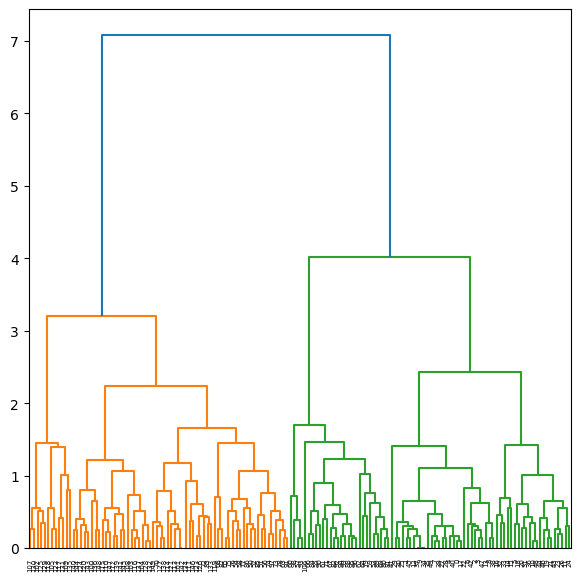
\includegraphics[width=0.35\textwidth]{Documentos Extra/Imagenes/complete_linkage.png}}
  \subfloat[Enlace simple]{
   \label{fig:single_linkage}
    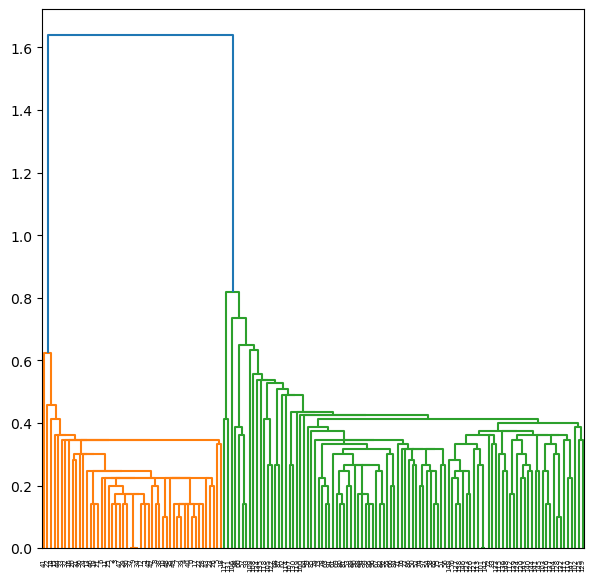
\includegraphics[width=0.35\textwidth]{Documentos Extra/Imagenes/single_linkage.png}}
 \caption{Diagramas obtenidos utilizando la biblioteca de Python Scikit-Learn}
 \label{fig:Dendogramas distintos enlaces }
\end{figure}
\end{column}
\end{columns}
\end{frame}
\begin{frame}{Métodos no supervisados}
\begin{columns}
\begin{column}{0.9\textwidth}

Como se ha dicho, los algoritmos particionales generan un único \emph{clustering} que se va modificando a lo largo de la ejecución del algoritmo.  

Para poder dar el algoritmo más importante de este tipo se necesita del siguiente concepto:

\begin{defi}
Se llama \emph{centroide} de un cluster $C_k,\enspace k=1,\ldots,K$ al vector de tamaño $p$ cuyas componentes son las medias de cada una de las variables de todas las observaciones del \emph{cluster} $C_k$:
\begin{equation}
\overline{x}_{jk}=\dfrac{1}{|C_k|}\sum_{i\in C_k}  x_{ij} \quad \forall j=1,\ldots, p
\end{equation}
\end{defi}
\end{column}
\end{columns}
\end{frame}

\begin{frame}{Métodos no supervisados}
\begin{columns}
\begin{column}{0.9\textwidth}

El algoritmo de $K$-medias se desarrolla de la siguiente manera:

 \begin{enumerate}
\item Se asignan a cada una de las observaciones en cada uno de los $K$ \emph{clusters}. Se calculan los centroides de dichos \emph{clusters}.
\item Se comprueba la distancia euclídea de cada una de las observaciones a los centroides de los \emph{clusters} y se reasignan las observaciones de acuerdo al  más cercano. Tras esto se recalculan los centroides.
\item Se repiten los dos pasos anteriores hasta que las asignaciones no cambien. 
\end{enumerate}
\end{column}
\end{columns}
\end{frame}

